\chapter{The~preliminaries}\label{chap:preliminaries}

This chapter consists of three sections. In the~first one (\ref{sec:wavelets}), we will briefly and formally describe the~main principle and usage of second generation wavelet transformation methods which are relevant for this thesis. In the~second one (\ref{sec:wavelets_cbdam}), we will compare the~compression inside C-BDAM and our method to these methods. Even though C-BDAM is based on the~same principle, it differs from these methods a~bit, so we will describe the basic differences. Then we will perform the~same basic comparison with our proposed method. Our method differs from the~described wavelet scheme a~bit more, see Section~\ref{sec:top-down} for the~details. Finally, in Section~\ref{sec:lossless_comp}, we describe two most common approaches to lossless data compression which are both used in Zlib - a~free compression library which we use in the~implementation of our method.

\section{The~introduction to second-generation wavelets}\label{sec:wavelets}
Basically, there are two generations of wavelets. The~first generation uses dilated and translated wavelet function~\cite{waveletsTutorial} for computation. The~second one uses filter banks to perform high-pass and low-pass filtering~\cite{waveletsLifting}. The~computational equivalency of these two approaches has been proven~\cite{waveletsEquiv}. For this work, the~second generation of discrete wavelet transform methods is most relevant, so we will briefly describe it in this section in order to give the~reader an~idea of the~wavelet concept which is referred to in many places of this thesis. We will base this description on 1-dimensional input data. We will also briefly describe how the~transition of the~principle to 2-dimensional data, such as images, can be performed.

Every method of this generation consists of just several subsequent applications of lifting onto the~input. The~lifting is the~basic step of the~method. It splits the~set of its input signal samples into two parts - low-pass (the~low frequency information) and high-pass (residuals, the~high frequency information). The~lifting is firstly applied on the~input set of signal samples and then is recursively applied to the~low-pass part produced by the~previous iteration until the~length of the~latest low-pass part is 1. In order to make this recursion possible, the~count of samples of the~original input of the~method must be a~certain power of two. If the~length of the input is $2^n$, the~method performs $n$ iterations of lifting. The~described successive application of lifting on smaller and smaller input is called the~bottom-up pass. We can imagine this as building a~pyramid of low-pass outputs the~first tier of which is the~input itself and every following higher tier is the~low-pass output of lifting applied to the~tier right below. Every tier is half the~width of the~previous one and after the~bottom-up pass, the~highest tier has the~width of 1 (Fig.~\ref{fig:wavelet_1d_pyramid}).

\begin{figure}
	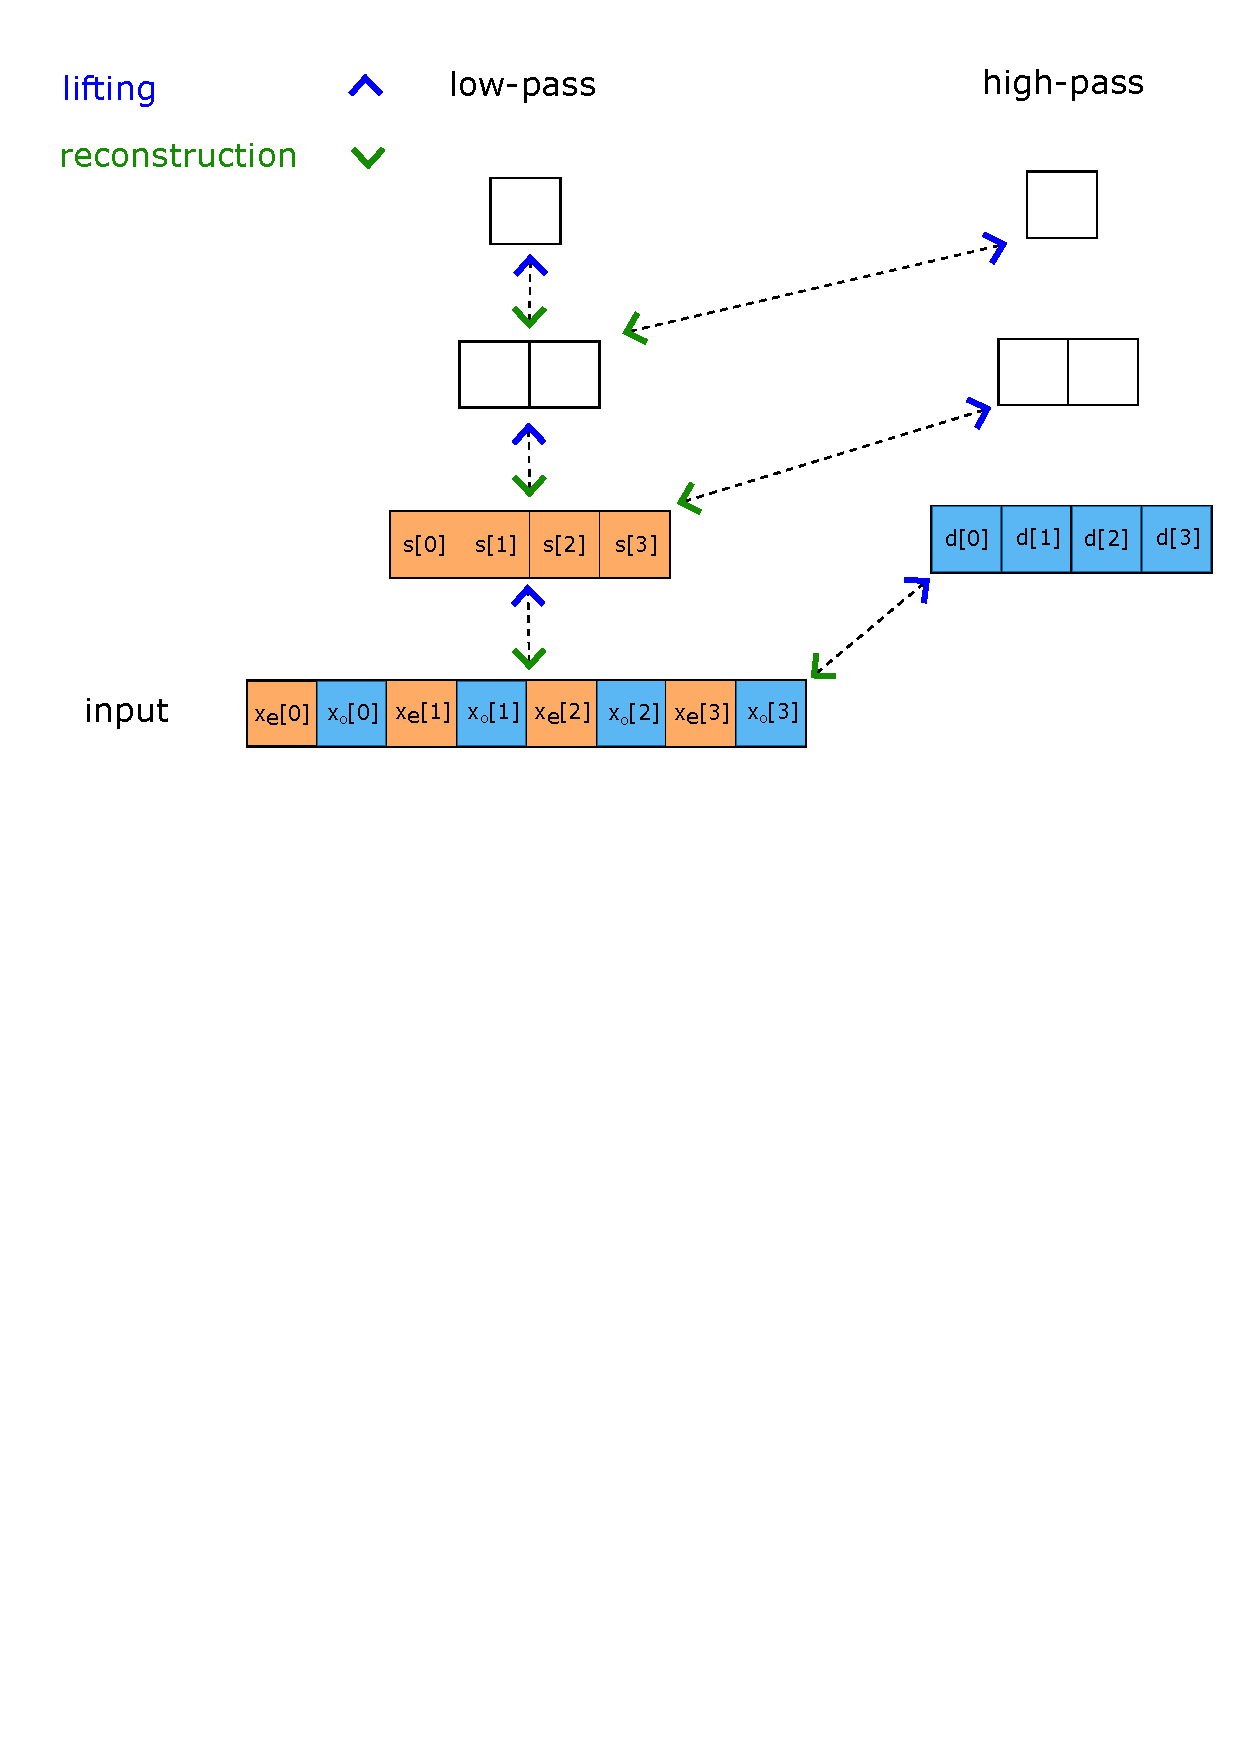
\includegraphics[trim={0 16cm 0 0}, clip, width=\textwidth]{figures/wavelet_1d_pyramid.pdf}\centering
	\caption{An~example of recursive wavelet decomposition of 1-dimensional data of samples. On the~left side, there is a~pyramid of low-pass tiers, the~bottom tier of which is the~input itself. On the~right side, there is the~corresponding pyramid of high-pass tiers. The~dashed lines represent both the~decomposition (lifting) inside the~first bottom-up pass (when following the~blue arrows) and the~inverse compositions (reconstruction) inside the~second top-down pass (when following the~green arrows). On the~input samples, it is also marked which samples form the~smaller low-pass part (the~orange ones) and the~smaller high-pass part (the~blue ones). The~orange ones are the~even ones, as the~indexing of samples is supposed to start at zero.}
	\label{fig:wavelet_1d_pyramid}
\end{figure}

After this bottom-up pass, we can perform the~inverse top-down pass. This pass does not know how the~produced pyramid looks, it only knows its highest tier, sized 1. However, it is supposed to be able to progressively reconstruct the~whole pyramid from the~top to the~bottom, only utilizing the~knowledge of the~high-pass information (Fig.~\ref{fig:wavelet_1d_pyramid}). Producing a~certain tier from the~previos one is called the~reconstruction which is the~exact opposite of lifting.

Now, let us briefly describe how this principle can be extended to 2-dimensional image data. Basically, this extension introduces just one change to the~described principle - when the~lifting is applied to an~image with dimension $2^n$, it produces four equally-sized outputs with dimension $2^{n-1}$: one low-pass part and three high-pass parts (Fig.~\ref{fig:wavelet_2d_pyramid}). Each of these high-pass parts contains different information - for example, the~first one might contain vertical edges, the~second one horizontal edges and the~third one diagonal edges. During the~subsequent reconstruction, all these four parts are used to produce the~larger low-pass part with twice better resolution.

\begin{figure}
	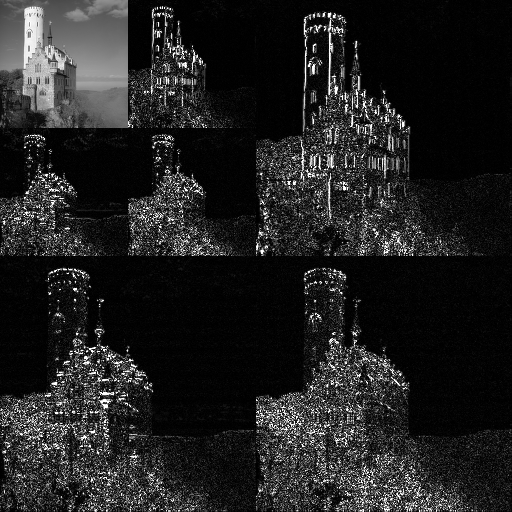
\includegraphics[width=\textwidth]{figures/wavelet_2d_pyramid.png}\centering
	\captionsource{An~example of recursive wavelet decomposition of 2-dimensional black-and-white image. The~sub-image at the~top-left corner stands for the~low-pass part after two iterations of lifting applied to the~input. The~original input is the~same as this sub-image, except for four times better resolution. The~neighbors of this low-pass part are its corresponding high-pass parts. The~top-right one of them contains vertical edges, the~bottom-left contains horizontal edges and the~bottom-right one contains diagonal edges. From these four top-left sub-images, twice as detailed low-pass part can be reconstructed. You can imagine this reconstruction as replacing these four sub-images with the~twice more detailed top-left sub-image. After this, we can merge it with the~remaining three largest high-pass parts to obtain the~original input.}
	{Wikimedia Commons~\cite{wavelet_2d_pyramid}}
	\label{fig:wavelet_2d_pyramid}
\end{figure}

What makes these decompositions and backward compositions useful is the~fact that the~top-down pass just needs the~high-pass information (residuals) to fully reconstruct the~input. This information tends to be sparse and input-dependent - the~smoother the~input, the~less high-pass information it contains. If we compress it well, we can save much storage space. Thus, if we want to store a~set of samples the~count of which is a~power of two in as little space as possible, we will not store the~samples directly, but we will store just the~compressed residuals produced by the~successive iterations of lifting applied to the~input. If we are not required to accurately reconstruct the~input, we can even decimate (quantize) the~residuals. Because this information often contains just details, its careful decimation does not deform the~reconstruction much and ensures better compression ratio. One more interesting fact is that the~residuals bound to lower tiers of the~pyramid carry finer details than those bound to the~higher ones. Thanks to this, the~more-detailed (larger) sets of residuals can be compressed more aggressively than the~less-detailed (smaller) ones. This is called progressive compression and it is used for example in JPEG standard~\cite{jpeg}.

In the~following lines, we will describe the~lifting and reconstruction steps in 1-dimensional domain more formally.
Let us say that the~lifting is given the~input samples $x_k$. It splits them into the~even ones:~$x_{2k} = x_e$ and the~odd ones:~$x_{2k+1} = x_o$. This splitting is not yet based on any frequency properties of the~samples, it is based just on their order. However, these two sets of samples will subsequently be modified, so that the~even ones will contain the~low-pass information and the~odd ones will become the~residuals - the~high-pass information. This will be performed with the~help of two operators: the~prediction operator $P$ and the~update operator $U$. $P$ will be used to produce the~residuals $d$ from $x_o$ and $U$ will be used to produce the~low-pass part $s$ from $x_e$.

Up to this point, just the~common properties of the~second-generation methods have been described. Now will come the~differences between them. The only thing they differ in is the~way they perform lifting and reconstruction. The way the~lifting step is performed clearly determines the~way how the~reconstruction is performed, as the~reconstruction must be the~exact inverse of lifting. The~lifting step varies in the~order in which the~operators $P$ and $U$ are applied. According to this, the~methods can be split into two main groups - the~prediction-first ones and the~update-first ones.

In the~prediction-first methods, the~prediction is applied first:

$$d = x_o - P(x_e)$$
$$s = x_e + U(d)$$

The~reconstruction must be the~exact inverse:

$$x_e = s - U(d)$$
$$x_o = d + P(x_e)$$

In the~update-first methods, the~update operator is applied first:

$$s = x_e + U(x_o)$$
$$d = x_o - P(s)$$

Here is how the~reconstruction looks then:

$$x_o = d + P(s)$$
$$x_e = s - U(x_o)$$

\section{Comparing the~wavelets to C-BDAM and our method}\label{sec:wavelets_cbdam}

In this section, we will briefly describe how the~compression inside C-BDAM and our method differ from the~basic second-generation wavelet scheme. Even thought C-BDAM works with 2D data, its lifting still has just two outputs, unlike in the~case of images. It is like it because of the~spatial arrangment of its height samples. In one iteration of lifting, a~half of samples is omitted (Fig.~\ref{fig:cbdam_lifting}). Its lifting is a~slight variation of the~update-first approach. The~main difference is that the~input to the~first update is not only $x_o$, but the~whole $x$. In addition, the~computation of $s$ is not the~summation of the~product of $x_e$ and $U$ anymore, because inside $U(x)$, $x_e$ is multiplied:

$$s = U(x)$$
$$d = x_o - P(s)$$

The~inverse reconstruction is then:

$$x_o = d + P(s)$$
$$x_e = U^{-1}(x)$$

Moreover, the~samples $x$ are regularly distributed in the~plane, so the~spliting into $x_o$ and $x_e$ no longer depends on the~indices of the~samples, but on their positions instead (Fig.~\ref{fig:cbdam_lifting}). Nevertheless, this is just a~formal difference which has no effect on the~computation. The~size of $x_o$ and $x_e$ is still half the~size of $x$ which is crucial to keep the~original form of 1D lifting. 

Note that if the~residuals $d$ were simply quantized after lifting and used in the~reconstructions inside the~second top-down pass, each step of the~reconstruction would increase the~maximum absolute deviation from the~original low-pass values produced in the~first bottom-up pass. To ensure that the~reconstructed values are within the~maximum-error bound from their corresponding values produced in the~first pass at each tier, the~residuals computed in the~first pass are slightly corrected according to the~actual values in another additional top-down pass. What is basically done is that we compare each reconstructed value with its target value. When it is too far from the~target value, its residual is shifted by a~multiple of the~quantization interval, so that the~resulting value is close enough to the~target value. Thanks to the~selection of the~quantization interval which respects the~set maximum-error bound, it is always possible to find such a~shift. The~following reconstruction (decompression) is again the~same top-down pass, except for the~fact that just the~corrected residuals are read, decompressed and used to progressively reconstruct the~data.

\begin{figure}
	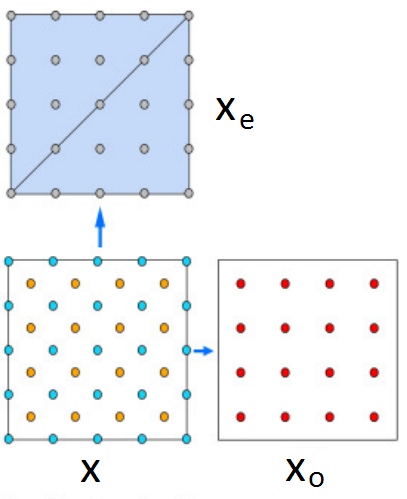
\includegraphics[width=0.28\textwidth]{figures/cbdam_lifting.png}\centering
	\captionsource{Lifting in C-BDAM - the~samples $x$ are split into the~even ones ($x_e$) which will become low-pass ($s$) and the~odd ones ($x_o$) which will become high-pass ($d$)}
	{C-BDAM~\cite{cbdam} (edited)}
	\label{fig:cbdam_lifting}
\end{figure}

The~method proposed in this thesis is update-first and uses the~whole $x$ as the~input to $U$, but has several differences: the~size of $x_e$ and thus $s$ is not half the~size of $x$, but one fourth of it instead, just like in the~2D example of images, as each four neighboring pixels of $x$ are collapsed into one inside $s$~(Fig.~\ref{fig:subst}). Additionally, the~lifting is not complete, because the~prediction operator is not applied there and the~computation of residuals is not performed there either. The~correct residuals which already ensure the~satisfaction of the~maximum-error bound constraint are computed directly in the~second top-down pass, also utilizing the~prediction operator. Similarly to C-BDAM, the~computations inside this pass are identical to the~reconstruction of the~data, except for the~fact that during the~reconstruction, the~residuals are not computed anymore. Additionally, the~prediction operator is applied multiple times in one step of the~reconstruction which is explained in Chapter~\ref{chap:details}. The~rationale behind all these differences is explained in Chapter.~\ref{chap:cbdam_comp}.

\section{Lossless compression}\label{sec:lossless_comp}

Lossless compression decreases the~data size without any information loss. It is often used to compress quantized residuals - the~output of wavelet transform. In this section, we briefly describe two main approaches to such compression - Huffman coding and dictionary compression. We do this because both these approaches are used in Zlib - a~publicly available lossless compression library which we use in our method to losslessly compress the~quantized residuals. We chose it because it achieved the~best compression ratios on our data from among all publicly available lossless compression libraries. It is also quite fast. It firstly applies LZ77 to the~data and then Huffman coding. Both these approaches basically profit from the~redundancy of data, but in different ways.

\subsection{LZ77 compression}\label{subsec:lz77}

This method is able to detect duplicite subsequences inside the~input which are relatively close to each other. It is very suitable for binary data. It reads the~input sequentially during the~compression. During this, it keeps track of the~last $N$ characters. We call this track the~sliding window, with $N$ being its length. In practice, $N$ is relatively large - 32KB in Zlib. 

We start at the~beginning of the~input stream, with an~empty window. Then, being at a~certain position, we examine the~data after the~window for the~longest continuous sequence beginning right after window which can also be found somewhere inside the~window. When we have found it, we just write a~triple ($D$, $L$, $C$) to the~output, with $D$ beingh the~distance of the~start of the~matching sequence found inside the~window to the~end of the~window, $L$ being the~length of the~sequence and $C$ being the~character in the~stream right after this sequence. Of course, it might happen that no such sequence is found - especially at the~very start - then both $D$ and $L$ will be 0. Note that $L$ might be greater than $D$ - in this case, when we reach the~end of the~window while trying to find the~longest match, we start again $D$ steps back from the~window's end. After outputting the triple ($D$, $L$, $C$), we move the~sliding window $L + 1$ steps forward. Note that this procedure works even for the~initial state - the~empty sliding window. In this case, (0, 0) is outputted, followed by the~first character of the~input stream. In this particular situation, (0, 0) can even be ommitted, as it has to always be written at the~beginning. Then, we repeat the~same matching of sequences again, as long as there is something to read. When we have reached the~end of the~stream, we write a~special end character at the~place of $C$.

The~decompression then works inversely as follows - it start with an~empty sliding window and then it starts reading all the~following triples ($D$, $L$, $C$). After reading each triple, it moves $D$ steps back from the~end of the~sliding window and copies $L$ following characters from the~current position to the~end of the~decompressed stream. If $L$ is greater than $D$, it goes back $D$ steps from the~window's end, or equally, it starts traversing the~output stream right after the~window's end, as in both cases, the~same characters will be found (the~first character which has been written after the~window was the~one located $D$ steps back from the~window's end). After writing all $L$ characters to the~decompressed stream, it writes $C$ to the~output stream, pushes the~sliding window forward by $L + 1$ steps and continues again with the~following triple. When it encounters the~special end character, it reads no more triples.

\subsection{Huffman coding}\label{subsec:huffman}

Huffman coding is a~form of prefix coding. It is usually used to compress data composed of characters. It might not be very suitable for arbitrary binary data, as it would most probably have to partition them into certain characters (bytes) in order to work. Thus, if the~binary data is actually composed of float numbers or something else distinct from characters, Huffman coding might not work very well and LZ77 is definitely a~better choice. However, in Zlib, Huffman coding is used to compress the~data produced by LZ77 - the~triples consisting of two natural numbers and one character - which can be easily interpreted as characters.

This algorithm starts by assigning a~certain weight to each of the~characters contained in the~data. The~more often the~character occurs, the~larger its weight should be. Then, according to these weights, it builds a~binary Huffman tree, with the~characters being the~leaf nodes of it. From each non-leaf node of the~tree, two edges go - they are marked as "0" and "1". The~marks of the~edges through which we have to traverse from the~root of the~tree to a~certain character form the~code of the~character in the~compressed stream. Ideally, the~greater the~weight of a~certain character, the~closer to the~root it should be, so the~shorter its code is.

With the~tree built, we can easily compress the~data. However, it remains a~question how exactly. The~main advantage of the~coding should be that the~more frequent characters have shorter codes, so we definitely would not profit from putting each code regularly into one or more bytes. But how to represent distinct lengths then? Should we somehow store the~code's length before the~code itself? Would not it be quite an overkill? 

Zlib comes with a~good solution - it constructs the~tree always in such way that no two characters have the~same code length. Thus, for the~subsequent decoding it is sufficient to store just the~lengths of the~codes. This is a~great solution, but did we need the~theory of Huffman coding here? This approach is practically equivalent to substituting each character with a~number. The~most frequent character is substituted by 1, the~second one by 2, etc. The~binary form of the~number is the~code of the~character. 


